\documentclass{article}
\usepackage{graphicx, tikz-cd, float, titlepic, booktabs} % Required for inserting images
\usepackage{amsmath, amssymb, amsthm, amsfonts, siunitx, physics, gensymb}
\AtBeginDocument{\RenewCommandCopy\qty\SI}
\usepackage[version=4]{mhchem}
\usepackage[most,many,breakable]{tcolorbox}
\usepackage{xcolor, fancyhdr, varwidth}
\usepackage[Glenn]{fncychap}
%Options: Sonny, Lenny, Glenn, Conny, Rejne, Bjarne, Bjornstrup
\usepackage{hyperref, cleveref}
\usepackage{icomma, enumitem} %comma as decimal and continue enumerate with [resume]
%%%%%%%%%%%%%%%%%%%%%%%%%%%%%%
% SELF MADE COLORS
%%%%%%%%%%%%%%%%%%%%%%%%%%%%%%
\definecolor{myg}{RGB}{56, 140, 70}
\definecolor{myb}{RGB}{45, 111, 177}
\definecolor{myr}{RGB}{199, 68, 64}
\definecolor{mytheorembg}{HTML}{F2F2F9}
\definecolor{mytheoremfr}{HTML}{00007B}
\definecolor{mylenmabg}{HTML}{FFFAF8}
\definecolor{mylenmafr}{HTML}{983b0f}
\definecolor{mypropbg}{HTML}{f2fbfc}
\definecolor{mypropfr}{HTML}{191971}
\definecolor{myexamplebg}{HTML}{F2FBF8}
\definecolor{myexamplefr}{HTML}{88D6D1}
\definecolor{myexampleti}{HTML}{2A7F7F}
\definecolor{mydefinitbg}{HTML}{E5E5FF}
\definecolor{mydefinitfr}{HTML}{3F3FA3}
\definecolor{notesgreen}{RGB}{0,162,0}
\definecolor{myp}{RGB}{197, 92, 212}
\definecolor{mygr}{HTML}{2C3338}
\definecolor{myred}{RGB}{127,0,0}
\definecolor{myyellow}{RGB}{169,121,69}
\definecolor{myexercisebg}{HTML}{F2FBF8}
\definecolor{myexercisefg}{HTML}{88D6D1}
%%%%%%%%%%%%%%%%%%%%%%%%%%%%%%%%%%%%%%%%%%%%%%%%%%%%%%%%%%%%%%%%%%%%%%
% Box environments for theorems and problems
%%%%%%%%%%%%%%%%%%%%%%%%%%%%%%%%%%%%%%%%%%%%%%%%%%%%%%%%%%%%%%%%%%%%%
\setlength{\parindent}{1cm}
%================================
% Question BOX
%================================
\makeatletter
\newtcbtheorem{question}{Opgave}{enhanced,
	breakable,
	colback=white,
	colframe=myb!80!black,
	attach boxed title to top left={yshift*=-\tcboxedtitleheight},
	fonttitle=\bfseries,
	title={#2},
	boxed title size=title,
	boxed title style={%
			sharp corners,
			rounded corners=northwest,
			colback=tcbcolframe,
			boxrule=0pt,
		},
	underlay boxed title={%
			\path[fill=tcbcolframe] (title.south west)--(title.south east)
			to[out=0, in=180] ([xshift=5mm]title.east)--
			(title.center-|frame.east)
			[rounded corners=\kvtcb@arc] |-
			(frame.north) -| cycle;
		},
	#1
}{def}
\makeatother
%================================
% DEFINITION BOX
%================================

\newtcbtheorem[]{Definition}{Definition}{enhanced,
	before skip=2mm,after skip=2mm, colback=red!5,colframe=red!80!black,boxrule=0.5mm,
	attach boxed title to top left={xshift=1cm,yshift*=1mm-\tcboxedtitleheight}, varwidth boxed title*=-3cm,
	boxed title style={frame code={
					\path[fill=tcbcolback]
					([yshift=-1mm,xshift=-1mm]frame.north west)
					arc[start angle=0,end angle=180,radius=1mm]
					([yshift=-1mm,xshift=1mm]frame.north east)
					arc[start angle=180,end angle=0,radius=1mm];
					\path[left color=tcbcolback!60!black,right color=tcbcolback!60!black,
						middle color=tcbcolback!80!black]
					([xshift=-2mm]frame.north west) -- ([xshift=2mm]frame.north east)
					[rounded corners=1mm]-- ([xshift=1mm,yshift=-1mm]frame.north east)
					-- (frame.south east) -- (frame.south west)
					-- ([xshift=-1mm,yshift=-1mm]frame.north west)
					[sharp corners]-- cycle;
				},interior engine=empty,
		},
	fonttitle=\bfseries,
	title={#2},#1}{def}
\newtcbtheorem[]{definition}{Definition}{enhanced,
	before skip=2mm,after skip=2mm, colback=red!5,colframe=red!80!black,boxrule=0.5mm,
	attach boxed title to top left={xshift=1cm,yshift*=1mm-\tcboxedtitleheight}, varwidth boxed title*=-3cm,
	boxed title style={frame code={
					\path[fill=tcbcolback]
					([yshift=-1mm,xshift=-1mm]frame.north west)
					arc[start angle=0,end angle=180,radius=1mm]
					([yshift=-1mm,xshift=1mm]frame.north east)
					arc[start angle=180,end angle=0,radius=1mm];
					\path[left color=tcbcolback!60!black,right color=tcbcolback!60!black,
						middle color=tcbcolback!80!black]
					([xshift=-2mm]frame.north west) -- ([xshift=2mm]frame.north east)
					[rounded corners=1mm]-- ([xshift=1mm,yshift=-1mm]frame.north east)
					-- (frame.south east) -- (frame.south west)
					-- ([xshift=-1mm,yshift=-1mm]frame.north west)
					[sharp corners]-- cycle;
				},interior engine=empty,
		},
	fonttitle=\bfseries,
	title={#2},#1}{def}

\newtcbtheorem{theo}%
    {Theorem}{}{theorem}
\newtcolorbox{prob}[1]{colback=red!5!white,colframe=red!50!black,fonttitle=\bfseries,title={#1}}
%================================
% NOTE BOX
%================================

\usetikzlibrary{arrows,calc,shadows.blur}
\tcbuselibrary{skins}
\newtcolorbox{note}[1][]{%
	enhanced jigsaw,
	colback=gray!20!white,%
	colframe=gray!80!black,
	size=small,
	boxrule=1pt,
	title=\textbf{Note:},
	halign title=flush center,
	coltitle=black,
	breakable,
	drop shadow=black!50!white,
	attach boxed title to top left={xshift=1cm,yshift=-\tcboxedtitleheight/2,yshifttext=-\tcboxedtitleheight/2},
	minipage boxed title=1.5cm,
	boxed title style={%
			colback=white,
			size=fbox,
			boxrule=1pt,
			boxsep=2pt,
			underlay={%
					\coordinate (dotA) at ($(interior.west) + (-0.5pt,0)$);
					\coordinate (dotB) at ($(interior.east) + (0.5pt,0)$);
					\begin{scope}
						\clip (interior.north west) rectangle ([xshift=3ex]interior.east);
						\filldraw [white, blur shadow={shadow opacity=60, shadow yshift=-.75ex}, rounded corners=2pt] (interior.north west) rectangle (interior.south east);
					\end{scope}
					\begin{scope}[gray!80!black]
						\fill (dotA) circle (2pt);
						\fill (dotB) circle (2pt);
					\end{scope}
				},
		},
	#1,
}

%%%%%%%%%%%%%%%%%%%%%%%%%%%%%%%%%%%%%%%%%%%%%%%%%%%%%%%%%%%%%%%%%
% SELF MADE COMMANDS
%%%%%%%%%%%%%%%%%%%%%%%%%%%%%%
\newcommand{\sol}{\setlength{\parindent}{0cm}\textbf{\textit{Løsning:}}\setlength{\parindent}{1cm}}
%%%%%%%%%%%%%%%%%%%%%%%%%%%%%%%%%
\usepackage[danish]{babel}
\usepackage[tmargin=2cm,rmargin=1in,lmargin=1in,margin=0.85in,bmargin=2cm,footskip=.2in]{geometry}\pagestyle{fancy}
\lhead{Minrui Kevin Zhou 2.b}
\rhead{Matematikaflevering 20}

\title{Aflevering 20\\
{\Large \textbf{2.b mat A}}}
\author{Kevin Zhou}
\date{November 2023}

\begin{document}
\maketitle
\section*{Bedømmelseskriterier:}
\begin{itemize}
    \setlength\itemsep{3cm}
    \Large
    \item  Redegørelse og dokumentation for metode
    \item Figurer, grafer og andre illustrationer
    \item Notation og layout
    \item Formidling og forklaring
\end{itemize}
\pagebreak

\begin{question}{Opgave 7}{}
 I \cref{fig:hund} ses en rektangulær løbegård til en hund.  
Løbegården skal bygges op ad en mur,
og de tre øvrige sider skal dannes af et $20 \;\unit{m} $ langt hegn. Løbegardens længde betegnes med $y$, og løbegårdens bredde betegnes med $x$.
Bestem $y$ udtrykt ved $x$. Bestem $x$, så arealet af løbegården bliver størst muligt.
\end{question}
\begin{figure}[H]
\begin{center}
  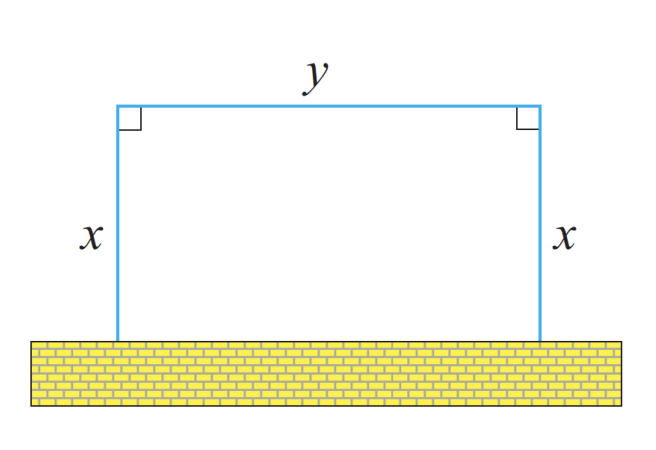
\includegraphics[scale=0.5]{Hund.png}
\end{center}
\caption{Løbegård til hunden}
\label{fig:hund}
\end{figure}
\sol \\ 
Siden de tre sider skal dannes af et $20 \;\unit{m  } $ langt hegn, så må følgende gælde. 
\[
2x+y=20 \iff y=20-2x
\] 
Arealet af løbegården som funktion af $x$, $A:\;]0;10[\;\to \mathbb{R}$ må da være bestemt ved
\[
A(x)=x\cdot (20 - 2x)=-2x^2+20x.
\] 
Vi differentierer funktionen og sætter lig med nul.
\begin{equation*}
\begin{split}
  \dv{A}{x}&=-4x+20 = 0 \\ 
  &\implies 4x=20 \\ 
  &\iff x=5
\end{split}
\end{equation*}
Vi ser da, at $5 \in Dm(A)$. For at se om $5$ er et maksimumssted, finder vi den dobbeltaflede funktion af $A$.
\[
A''(x)=\dv{x} (-4x + 20) = -4
\] 
$5$ være et maksimumssted, siden $A''(5)<0$. Altså er arealet af løbegården størst muligt, når $x$ er $5 \;\unit{m} $.

\begin{question}{Opgave 8}{}
  En kvægavler vil indhegne et stykke jord. Indhegningen skal være rektangulær, og ved hjælp af et hegn parallelt med det ene par sider skal den deles i to adskilte folde.
  Der er i alt $600$ meter hegn til rådighed.
Bestem det størst mulige areal af det indhegnede stykke jord.
\end{question}
\sol \\ 
Lad længden af siderne, der er parallele med hegnet, der deler indhegningen i to adskilte folde være betegnet med $x$.
Lad længden af hver af de to ortogonale sider til hegnet, der deler indhegningen i to adskilte folde være betegnet med $y$.
Så gælder der, at
\[
3x+2y=600 \implies y=\frac{600-3x}{2}=300 - \frac{3}{2} x
\] 
Arealet af det indhegnede stykke jord som funktion af $x$, $A:\;]0;200[\;\to \mathbb{R}$ må da være bestemt ved
\[
A=x\cdot y \implies A(x)=- \frac{3}{2}x^2 + 300x
\] 
Vi differentierer og sætter lig med 0.
\begin{equation*}
\begin{split}
  \dv{A}{x}&=-3x+300=0 \\ 
  &\implies 3x=300 \\ 
  &\iff x=100
\end{split}
\end{equation*}
Vi ser da, at $100 \in Dm(A)$. 
For at se om $100$ er et maksimumssted, finder vi den dobbeltaflede funktion af $A$.
\[
A''(x)=\dv{x} (-3x+300)=-3
\] 
Siden $A''(100)=-3<0$, så må $100$ være det globale maksimumssted. 
Vi finder nu arealet, når $x=100$.
\[
A(100)=- \frac{3}{2}(100)^2 + 300 \cdot 100=15000
\] 
Altså er det størst mulige areal af det indhegnede stykke jord $15000 \;\unit{m}^2 $.

\begin{question}{Opgave 9}{}
  En kasse uden låg har kvadratisk bund. Rumfanget af kassen er 32. 
På figuren i \cref{fig:kasse} betegner $x$ sidelængden i den kvadratiske bund, og $h$ betegner kassens højde.
Bestem $h$ udtrykt ved $x$ og bestem den værdi af $x$, som gør kassens samlede overfladeareal mindst muligt. 
\end{question}
\begin{figure}[H]
\begin{center}
  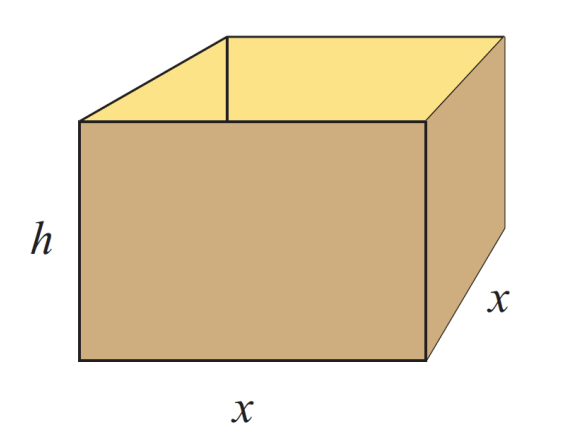
\includegraphics[scale=0.7]{Kasse.png}
\end{center}
\caption{Kasse uden låg}
\label{fig:kasse}
\end{figure}
\sol \\ 
Med hensyn til rumfanget af kassen, så kan vi bestemme $h$ udtrykt ved $x$.
\[
h\cdot x^2=32 \implies h=\frac{32}{x^2}
\] 
Overfladearealet af kassen er
\[
o=4\cdot hx + x^2=4\cdot \frac{32}{x} + x^2
\] 
Vi differentierer dette udtryk med hensyn til $x$ og sætter lig med 0.
\begin{equation*}
\begin{split}
  \dv{x} (x^2+4\cdot 32x^{-1})&=2x-4\cdot \frac{32}{x^2} = 0 \\
  &\implies x^3=64 \\ 
  &\iff x=\sqrt[3]{64}=4
\end{split}
\end{equation*}
Siden 
\[
\dv[2]{x} (x^2 + 4\cdot 32x^{-1})=\frac{256}{x^3}+2
\] 
og når $x=4$:
\[
\dv[2]{x} (x^2 + 4\cdot 32x^{-1})=6>0
\] 
så må $4$ være det globale minimumssted.
Altså er kassens samlede overfladeareal mindst muligt, når $x=4$.

\begin{question}{Opgave 10}{}
En $7 \;\unit{m} $ lang stige er placeret op ad en lodret mur.
Stigens røringspunkt med jorden benævnes $A$, og stigens røringspunkt med muren benævnes $B$. 
Afstanden mellem stigen og murens fod benævnes $d$. 
Afstanden mellem murens fod og stigens fod benævnes med $x$, og det oplyses, at $0<x<7$.
\begin{itemize}
  \item[a.] Gør rede for, at $|BC|=\sqrt{49-x^2} $, og benyt dette til at vise, at $d=\frac{x\cdot \sqrt{49-x^2} }{7}$. 
  \item[b.] Bestem $x$, så $d$ bliver størst mulig. 
\end{itemize}
\end{question}
\begin{figure}[H]
\begin{center}
  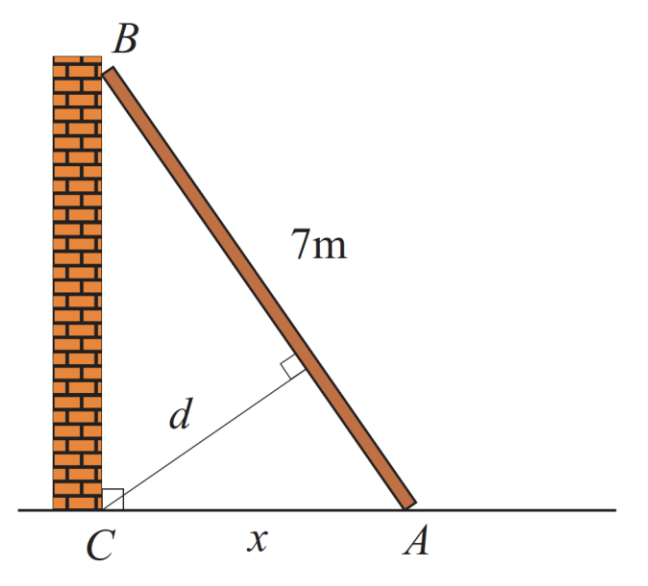
\includegraphics[width=0.5\textwidth]{mur.png}
\end{center}
\caption{Stige op af en lodret mur som i opgaven}
\label{fig:mur}
\end{figure}

\sol \\ 
\textbf{a.} Ved at bruge Pythagoras' læresætning kan vi se på \cref{fig:mur}, at
\[
\left|BC\right|=\sqrt{\left|AB\right|^2-\left|AC\right|^2} = \sqrt{49-x^2} 
\] 
Vi kan da kigge på arealet af trekanten for at finde et udtryk for $d$.
\begin{equation*}
\begin{split}
  A&=\frac{1}{2}\cdot \left|AB\right| \cdot d = \frac{1}{2} \cdot \left|BC\right| \cdot x\\
  &\implies 7 \cdot d = \sqrt{49-x^2} \cdot x\\ 
  &\iff d=\frac{x\cdot \sqrt{49-x^2} }{7}
\end{split}
\end{equation*}
hvilket var, hvad vi skulle vise. \\[1ex]
\textbf{b.} Vi differentierer udtrykket for $d$ fundet i \textbf{a.} med produktreglen og kædereglen.
\begin{equation*}
\begin{split}
  \dv{x} \left(\frac{x\cdot \sqrt{49-x^2} }{7}\right)&=\frac{1}{7} \left(\sqrt{49-x^2} + x\cdot \dv{x} (\sqrt{49-x^2} )\right) \\ 
  &= \frac{1}{7} \left(\sqrt{49-x^2} + x\cdot \frac{-2x}{2 \sqrt{49-x^2} } \right)\\ 
  &= \frac{49-2x^2}{7 \sqrt{49-x^2} }
\end{split}
\end{equation*}
Vi sætter dette lig med 0 og løser for $x$.
\begin{equation*}
\begin{split}
  \frac{49-2x^2}{7 \sqrt{49-x^2} }= 0 &\iff 49 - 2x^2=0 \\ 
  &\iff x^2=\frac{49}{2}\\ 
  &\iff x=-\frac{7}{\sqrt{2} } \lor x=\frac{7}{\sqrt{2} }
\end{split}
\end{equation*}
Dog siden $x \in \mathbb{R}^+$, så må $x$ være positiv. 
Vi finder det dobbeltdifferentierer udtrykket for $d$ med CAS (se \cref{fig:CAS}). 
\[
\dv[2]{x}\left(\frac{x\cdot \sqrt{49-x^2} }{7}\right)=\frac{x(2x^2-147)}{7(49-x^2)^{3/2}}
\] 
Når $x=\frac{7}{\sqrt{2} }$, så får vi med CAS (se \cref{fig:CAS}), at
\[
\dv[2]{x}\left(\frac{x\cdot \sqrt{49-x^2} }{7}\right)=-\frac{4}{7}<0
\] 
Altså må $\frac{7}{\sqrt{2} }$ være det globale maksimumssted med hensyn til $d$. 
Det vil sige, at $d$ er størst mulig, når $x=\frac{7}{\sqrt{2} }$. 
\begin{figure}[H]
\begin{center}
  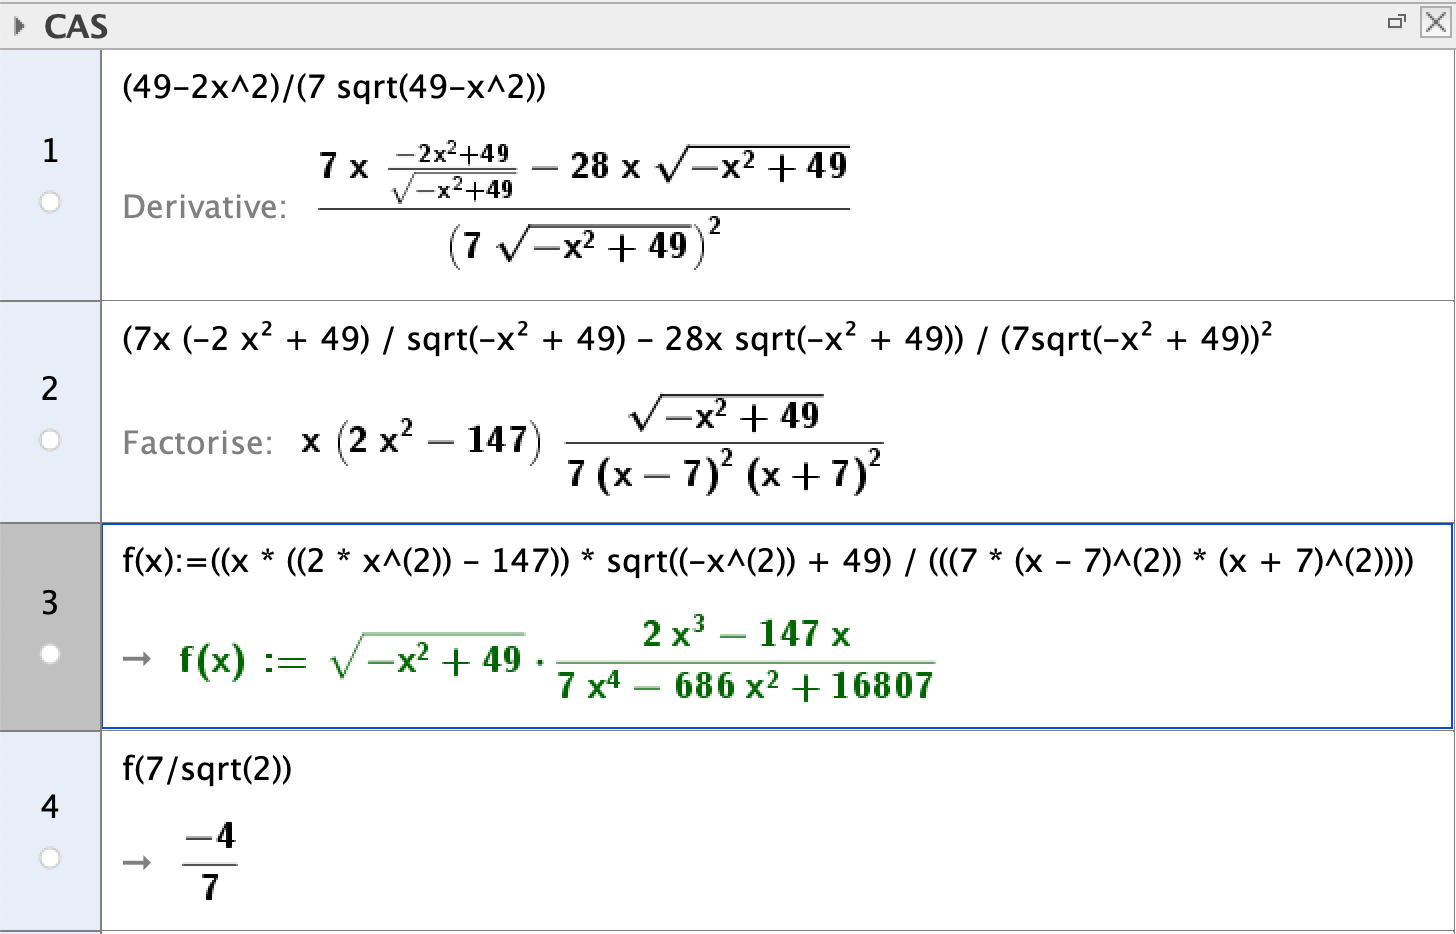
\includegraphics[width=0.7\textwidth]{CAS.png}
\end{center}
\caption{Måden, hvorpå CAS er brugt til regning af ovenstående}
\label{fig:CAS}
\end{figure}

\end{document}
